\section{The Intel 486}
\par
Checkout \cw{https://en.wikipedia.org/wiki/NEAT\_chipset} for details of motherboard.\\
\par

\cfullimage{PX486P3/b-486-px486p3}{}
\cfullimage{PX486P3/px486p3_drawing}{}
\section{Intel 486}
By may 1992, the Intel 386 was being replaced by a new version, the 486. The increase in operatin frequency was substancial for the high end model running at 50Mhz but most 486 ran at the same speed at the 386: 25Mhz and 33Mhz. The revolutionary design of the CPU.\\
\fullimage{i486DX.png}
\par
\begin{figure}[H]
\centering
  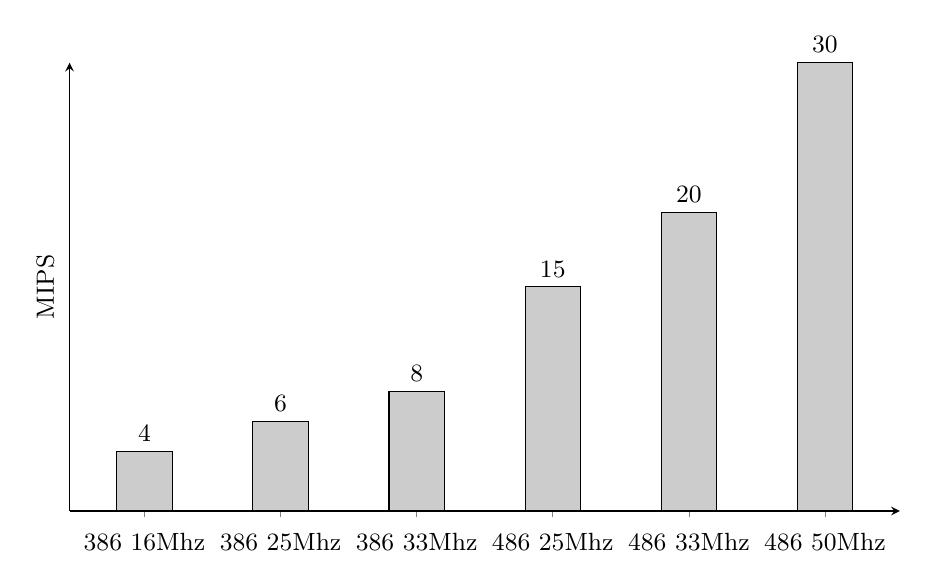
\begin{tikzpicture}[font=\small]
    \begin{axis}[
      width=1.0\textwidth,
      height=0.6\textwidth,
      ybar,
      bar width=20pt,
      ylabel={MIPS},
      ymin=0,
      ytick=\empty,
      xtick=data,
      axis x line=bottom,
      axis y line=left,
      enlarge x limits=0.11,
      symbolic x coords={386 16Mhz,386 25Mhz,386 33Mhz,486 25Mhz,486 33Mhz,486 50Mhz},
      xticklabel style={anchor=base,yshift=-\baselineskip},
      nodes near coords={\pgfmathprintnumber\pgfplotspointmeta}
    ]
      \addplot[fill=black!20,draw=black] coordinates {
        (386 16Mhz,4)
        (386 25Mhz,6)
        (386 33Mhz,8)
        (486 25Mhz,15)
        (486 33Mhz,20)
        (486 50Mhz,30)
      };
    \end{axis}
   
   \end{tikzpicture}
   \caption{Comparison\protect\footnotemark of CPUs with MIPS \protect\footnotemark.}
 \end{figure}
\footnotetext{Source: "Roy Longbottom's PC Benchmark Collection: http://www.roylongbottom.org.uk/mips.htm".}













\subsection{Floating Point Unit}


\subsection{Pipeline}



\begin{figure}[H]
\centering
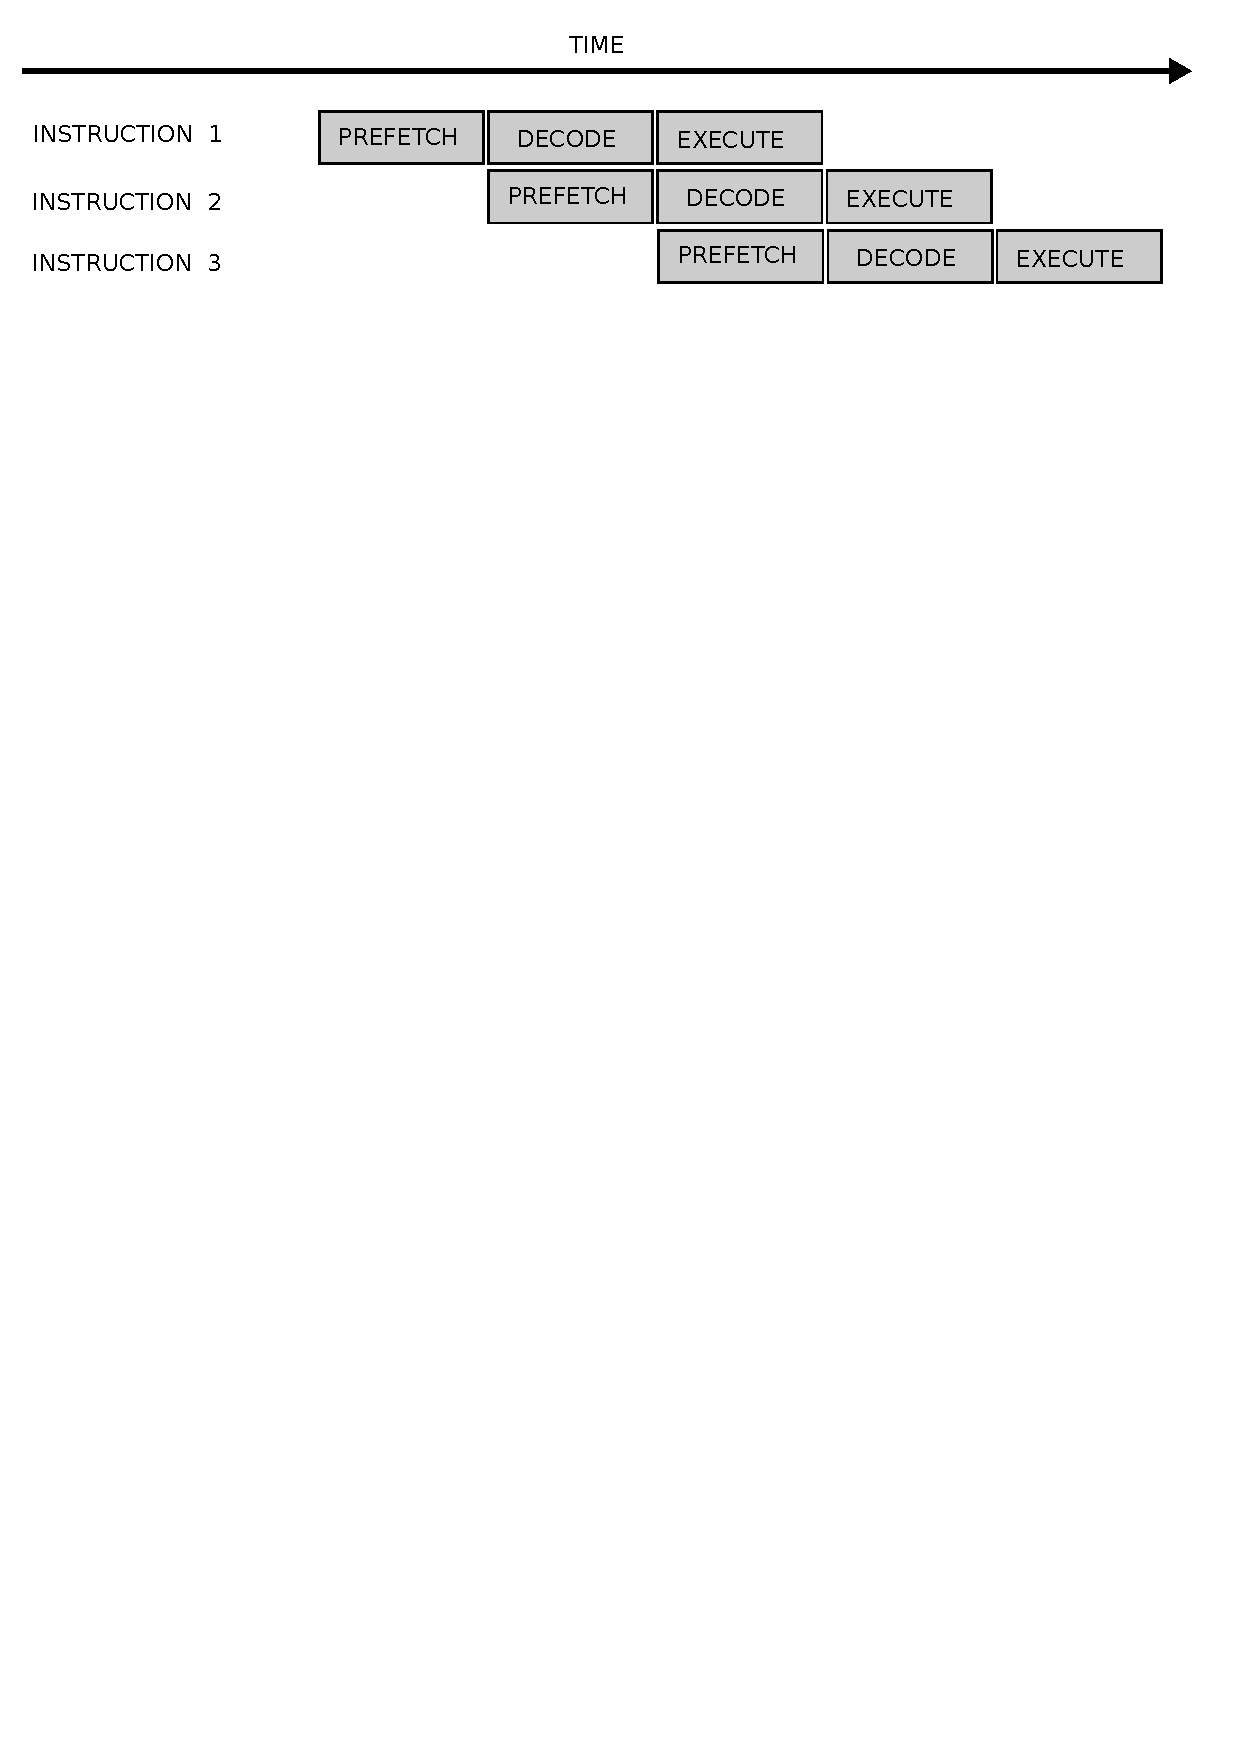
\includegraphics[width=\textwidth]{drawings/386_instruction_pipeline.pdf}
\caption{386 pipeline in Intel documentation.}
\end{figure}
\par


\begin{figure}[H]
\centering
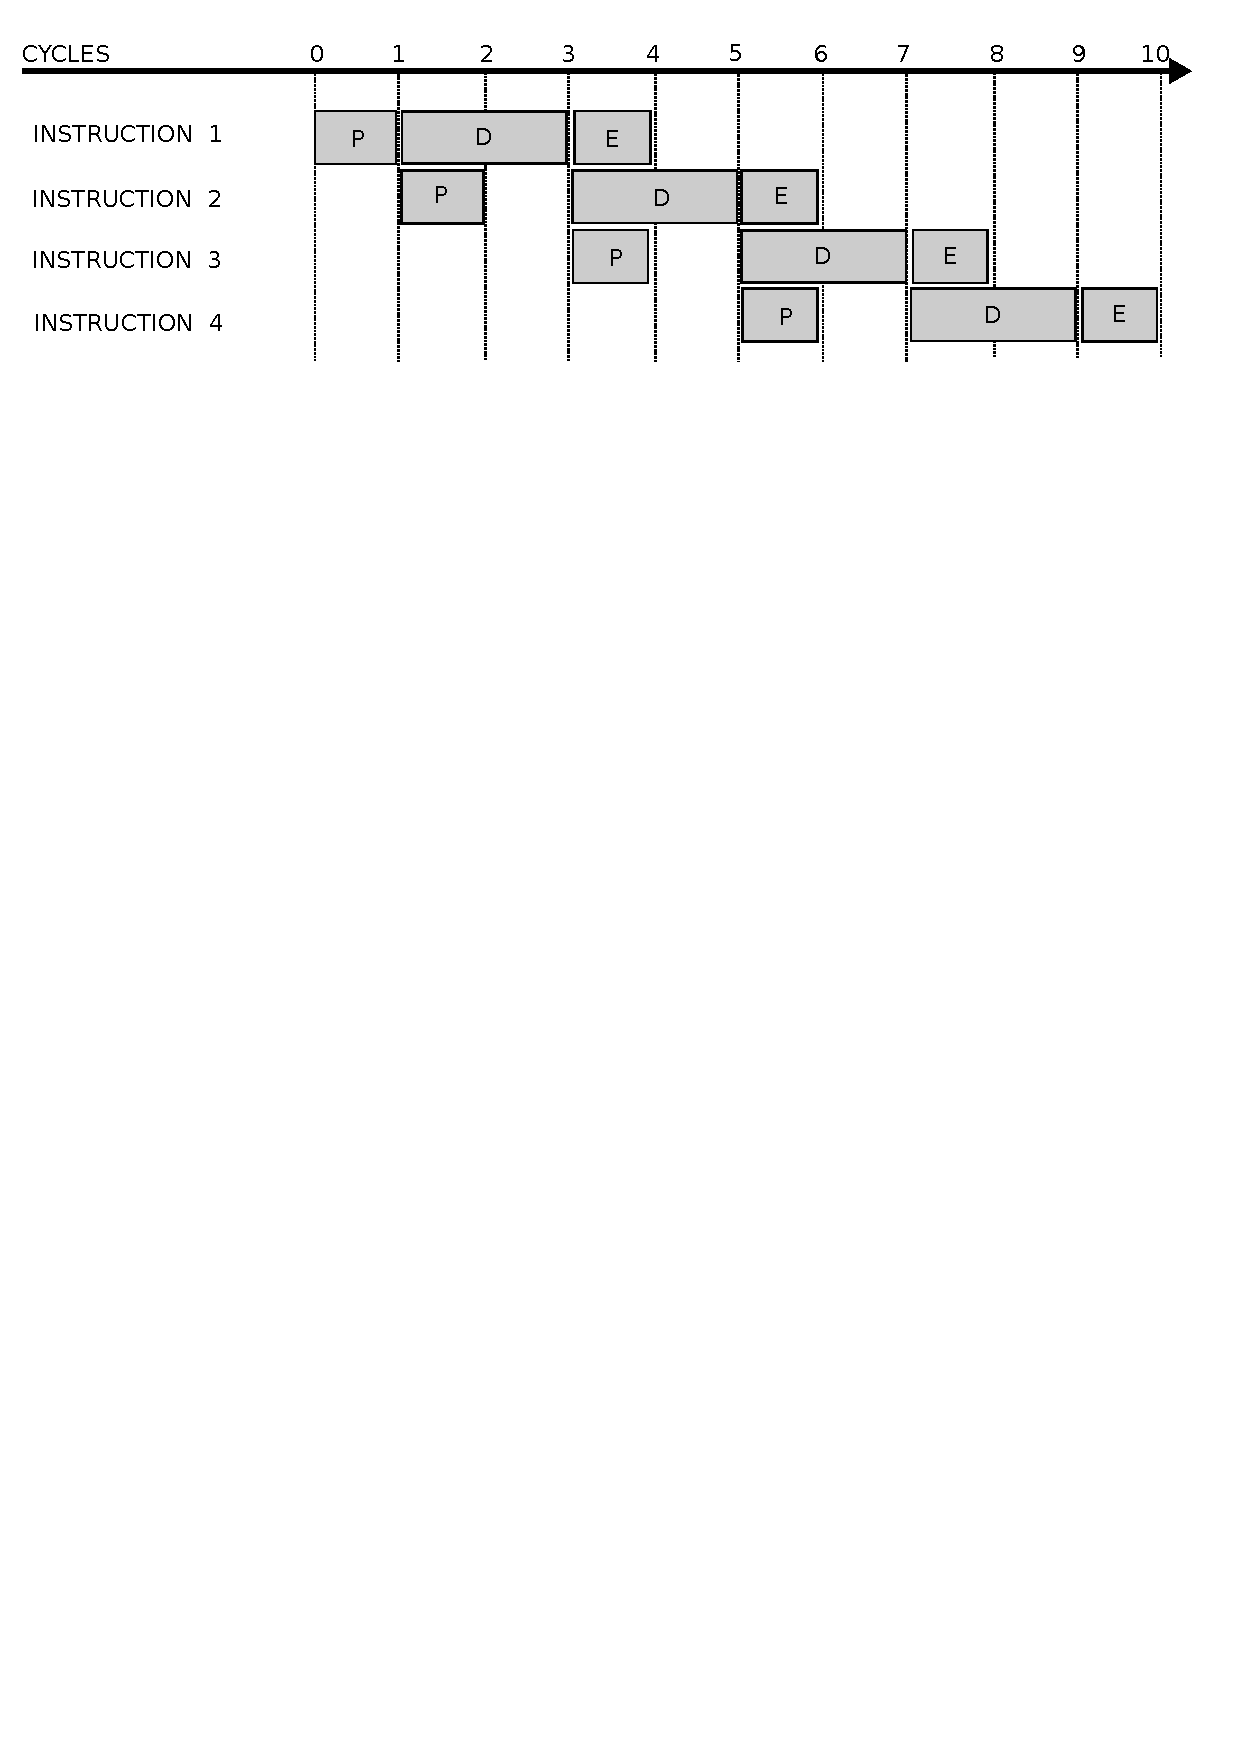
\includegraphics[width=\textwidth]{drawings/actual_386_instruction_pipeline.pdf}
\caption{386 pipeline: Two cycles per instruction.}
\end{figure}
\par

\begin{figure}[H]
\centering
\includegraphics[width=\textwidth]{drawings/actual_486_instruction_pipeline.pdf}
\caption{486 pipeline: One cycle per instruction.}
\end{figure}
\par

\subsection{Cache L1}
four-way set-associative write through.\\

\subsection{Cache L2}
Bla
\subsection{Precaching (cachelines) Netburst}
Bla













\section{Overdrive, 486 DX2 66Mhz}
\begin{figure}[H]
\centering
  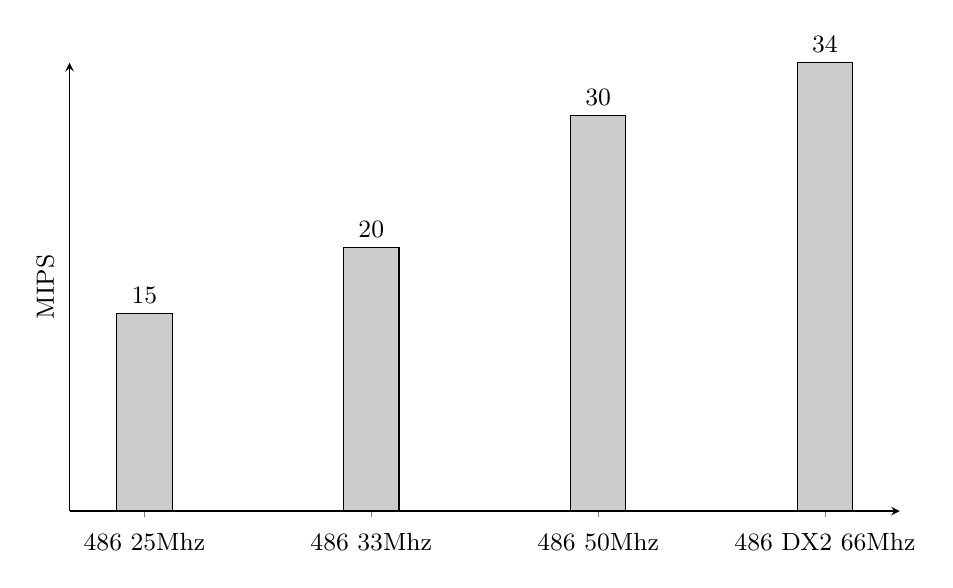
\begin{tikzpicture}[font=\small]
    \begin{axis}[
      width=1.0\textwidth,
      height=0.6\textwidth,
      ybar,
      bar width=20pt,
      ylabel={MIPS},
      ymin=0,
      ytick=\empty,
      xtick=data,
      axis x line=bottom,
      axis y line=left,
      enlarge x limits=0.11,
      symbolic x coords={486 25Mhz,486 33Mhz,486 50Mhz,486 DX2 66Mhz},
      xticklabel style={anchor=base,yshift=-\baselineskip},
      nodes near coords={\pgfmathprintnumber\pgfplotspointmeta}
    ]
      \addplot[fill=black!20,draw=black] coordinates {
        (486 25Mhz,15)
        (486 33Mhz,20)
        (486 50Mhz,30)
        (486 DX2 66Mhz,34)
      };
    \end{axis}
   
   \end{tikzpicture}
   \caption{Comparison\protect\footnotemark of CPUs with MIPS \protect\footnotemark.}
 \end{figure}
\footnotetext{Source: "Roy Longbottom's PC Benchmark Collection: http://www.roylongbottom.org.uk/mips.htm".}

four-way set-associative write back.\\